\chapter{Unterräume, Projektionsoperatoren und Messung als Verschränkung}

Der Satz von Bell hat zwei Fragen offen gelassen. Was bleibt von der Verschränkung, wenn ein Teil eines Paars gestört, absorbiert oder gemessen wird? Und wodurch wird eine gewöhnliche Wechselwirkung genau zu einer Messung? Der Weg zur Antwort führt durch elementare lineare Algebra. Eigenschaften sind Unterräume, Wahrscheinlichkeiten Erwartungswerte von Projektoren, und ein Messgerät ist ein weiteres Quantensystem, mit dem das Objekt verschränkt wird.

\section{Ausgangsfrage: Verschränkung, Lokalität und Messung}

Nehmen wir an, ein Singulettzustand sei in zwei weit voneinander entfernte Teile getrennt worden und einer davon werde gemessen. Muss die Quantenfeldtheorie einen virtuellen Austausch zwischen ihnen beschreiben? Auf der entfernten Seite geschieht nichts Nachweisbares, und dort kommt keine nutzbare Nachricht an. Man kann lokal einen Spin mithilfe eines Magnetfelds drehen und dadurch die konkrete Form des gemeinsamen Zustands verändern, während der Verschränkungsgrad unter dieser lokalen Operation unverändert bleibt. Quantitative Maße für Verschränkung werden später behandelt; hier geht es zunächst darum, dass zwei Systeme, die nicht mehr miteinander wechselwirken, ihre gemeinsame Verschränkung nicht allein durch eine auf eine Seite beschränkte Operation ändern können.

\begin{classroomqa}\lecturetimestamp{00:00:22}\audiencequestion{Erfordert eine Messung an einem Teil eines raumartig getrennten Singuletts einen virtuellen Austausch mit dem anderen?}\lecturerresponse{Auf der anderen Seite findet kein nachweisbarer Austausch statt. Eine lokale Operation kann einen Faktor drehen und die Form ändern, in der der gemeinsame Zustand dargestellt wird; für sich genommen kann sie aber weder eine Nachricht übermitteln noch die über die räumliche Trennung hinweg bestehende Verschränkung ändern.}\end{classroomqa}

Das erzwingt einen umfassenderen Begriff davon, was als Partner gilt. Fällt ein Teil eines verschränkten Paars in ein Schwarzes Loch, hört der andere nicht auf, verschränkt zu sein; er wird mit den Freiheitsgraden des Schwarzen Lochs und nach dessen Verdampfung mit der ausgesandten Strahlung verschränkt. Dazu braucht es kein Schwarzes Loch. Lässt man einen Teil eines verschränkten Paars in eine Badewanne fallen und heftig mit dem Wasser vermischen, kann seine individuelle Identität im Vielteilchenzustand verloren gehen. Dennoch bleibt das entfernte Teilchen mit der Badewanne als Ganzem und schließlich mit dem entweichenden Wasserdampf verschränkt.

Dabei geht es nicht nur um Fortbestehen, sondern auch um Umkehrbarkeit. Wenn eine Wechselwirkung Verschränkung erzeugen kann, kann sie sie prinzipiell auch rückgängig machen. Eine Entschränkung ist möglich, aber nur, wenn die Systeme wieder in Kontakt kommen und erneut miteinander wechselwirken. Was in der einen Richtung geschehen kann, kann auch in der anderen geschehen.

\begin{classroomqa}\lecturetimestamp{00:04:45}\audiencequestion{Bleiben die Elektronen verschränkt, wenn beide Spins eines verschränkten Paars gemessen werden? Kann bereits eine Messung sie entschänken?}\lecturerresponse{Die Messungen können ihre gegenseitige Verschränkung aufheben, und eine einzige Messung kann dafür ausreichen. Um zu verstehen, was diese Aussage bedeutet, statt lediglich einen Kollaps zu behaupten, müssen wir Beobachtung als Wechselwirkung zwischen dem System und einem Aufzeichnungsgerät beschreiben.}\end{classroomqa}

Diese Frage gibt die Richtung vor: Beobachtung, Kollaps des Wellenpakets und Verschränkung miteinander zu verbinden. Bevor wir uns ihr zuwenden, brauchen wir jedoch eine klarere Darstellung von Unterräumen und Projektionsoperatoren, die nicht mehr mathematische Mittel einsetzt, als die Argumentation erfordert.

\section{Dimension, lineare Abhängigkeit und Orthonormalbasen}

Wir bleiben daher zunächst bei endlichdimensionalen Vektorräumen mit Bra- und Ket-Vektoren sowie einem Skalarprodukt. Susskind beginnt so elementar wie möglich. Er definiert die Dimension nicht dadurch, dass man die Komponenten eines Spaltenvektors zählt. Stattdessen definiert er sie abstrakt: Die Dimension eines Vektorraums ist die maximale Anzahl linear unabhängiger Vektoren, die sich darin finden lassen.

Eine Menge \(\{|v_i\rangle\}\) ist also linear unabhängig, wenn die Relation
\begin{equation}
\sum_i c_i |v_i\rangle = 0
\end{equation}
erzwingt, dass alle Koeffizienten \(c_i\) verschwinden. Gleichbedeutend damit ist, dass sich keiner der Vektoren als Linearkombination der übrigen schreiben lässt.

Entscheidend ist hier, dass Orthogonalität nicht dasselbe ist wie Unabhängigkeit. In drei Dimensionen kann es drei Vektoren geben, die überhaupt nicht orthogonal und dennoch linear unabhängig sind. Es kommt darauf an, ob sich einer von ihnen aus den beiden anderen zusammensetzen lässt. In einer zweidimensionalen Ebene muss dagegen jeder dritte Vektor von den ersten beiden linear abhängig sein.

\begin{figure}[htbp]\centering
\includegraphics[width=0.56\textwidth]{lecture_06_figure_02.png}\caption{Drei an der Tafel eingezeichnete Vektoren. Die Vorlesung nutzt diese Skizze, um Orthogonalität und lineare Unabhängigkeit voneinander abzugrenzen und anschließend hervorzuheben, dass in einer Ebene ein dritter Vektor von den ersten beiden abhängig ist.}\lectureframe{00:09:35}\end{figure}

\begin{figure}[htbp]\centering
\begin{tikzpicture}[scale=1.2]
\draw[->] (0,0) -- (2.3,0);
\draw[->] (0,0) -- (2.0,2.0);
\draw[->] (0.35,0.95) -- (1.05,1.45);
\fill (0,0) circle (1.2pt);
\end{tikzpicture}\caption{Eine vereinfachte Rekonstruktion der Tafelskizze. Die genaue Koeffizientenrelation lässt sich allein aus dem Bild nicht bestimmen; die geometrische Aussage ist, dass ein dritter Vektor in einer zweidimensionalen Ebene nicht unabhängig ist.}\end{figure}

Das ist der Punkt der Skizze. Ist der Raum zweidimensional, beträgt die maximale Anzahl linear unabhängiger Vektoren zwei. Ist er dreidimensional, beträgt sie drei. Allgemeiner gilt: Hat der Raum die Dimension \(d\), dann lassen sich bei gegebenem Skalarprodukt \(d\) paarweise orthogonale Einheitsvektoren finden, die ihn aufspannen. Das sind Basisvektoren. Susskind sagt ausdrücklich, dass er diesen Satz hier nicht beweisen wird. Ihm geht es nur um die Folgerung: Sobald eine solche Basis existiert, lässt sich jeder Vektor des Raums nach ihr entwickeln.

\begin{classroomqa}\lecturetimestamp{00:10:58}\audiencequestion{Ist die Zahl der räumlichen Freiheitsgrade gleich der Dimension des Zustandsraums?}\lecturerresponse{Nein. Ein Teilchen, das sich in einem Raum bewegt, hat drei räumliche Koordinaten, aber eine sehr große Zahl paarweise orthogonaler Quantenzustände. Die Dimension des Konfigurationsraums und die Dimension des Hilbertraums sind verschiedene Begriffe; endlichdimensionale Beispiele dienen hier lediglich dazu, die Logik klar herauszuarbeiten.}\end{classroomqa}

\section{Basisentwicklung, Dyaden und Vollständigkeitsrelation}

Wählen wir nun eine Orthonormalbasis \(\{|n\rangle\}\) mit \(n=1,\dots,d\). Die Tafelanschrift ist an dieser Stelle besonders übersichtlich und knapp:

\begin{figure}[htbp]\centering
\includegraphics[width=0.62\textwidth]{lecture_06_figure_03.png}\caption{Orthonormalbasis und Entwicklung eines beliebigen Zustands.}\lectureframe{00:14:15}\end{figure}

Wir schreiben
\begin{align}
\langle m|n\rangle &= \delta_{mn}, \\
|\psi\rangle &= \sum_n a_n |n\rangle.
\end{align}
Hier ist \(\delta_{mn}\) das Kronecker-Delta: Es ist \(1\) für \(m=n\) und andernfalls \(0\).

\paragraph{Herleitung.} Die Koeffizienten erhält man durch Projektion auf die Basis. Multiplizieren wir von links mit \(\langle m|\):
\begin{align}
\langle m|\psi\rangle
  &= \sum_n a_n \langle m|n\rangle \\
  &= \sum_n a_n \delta_{mn} \\
  &= a_m.
\end{align}
Damit sind die Koeffizienten einfach
\begin{equation}
a_m = \langle m|\psi\rangle.
\end{equation}
Der Koeffizient ist eine gewöhnliche komplexe Zahl und kann daher unverändert auf beiden Seiten des Kets stehen.

Setzen wir den Koeffizienten wieder in die Entwicklung ein, erhalten wir
\begin{equation}
|\psi\rangle = \sum_n |n\rangle \langle n|\psi\rangle.
\end{equation}
Das legt nahe, das Objekt \(|n\rangle\langle n|\) und allgemeiner \(|a\rangle\langle b|\) als Operator zu lesen. Genau das ist der nächste Schritt. Eine Dyade wirkt gemäß
\begin{equation}
\bigl(|a\rangle\langle b|\bigr)|\psi\rangle = \langle b|\psi\rangle\,|a\rangle.
\end{equation}
Das Bra liefert eine komplexe Zahl, das Ket die resultierende Richtung. So gelangt Susskind auf einfachem Weg von Vektoren zu Operatoren.

Betrachten wir nun die vorherige Entwicklung in Operatorform. Da
\begin{equation}
|\psi\rangle = \left(\sum_n |n\rangle\langle n|\right)|\psi\rangle
\end{equation}
für jedes \(|\psi\rangle\) gilt, muss der Operator in den Klammern die Identität sein:
\begin{equation}
\sum_n |n\rangle\langle n| = I.
\end{equation}
Dies ist die Vollständigkeitsrelation.

\begin{figure}[htbp]\centering
\includegraphics[width=0.60\textwidth]{lecture_06_figure_07.png}\caption{Die vollständige Vollständigkeitsrelation an der Tafel.}\lectureframe{00:18:30}\end{figure}

\begin{classroomqa}\lecturetimestamp{00:18:39}\audiencequestion{Müssen die Vektoren in der Vollständigkeitsrelation eine Basis bilden?}\lecturerresponse{Ja. In der Herleitung wurden sowohl die Normierung als auch die gegenseitige Orthogonalität vorausgesetzt, und die Summe muss über eine vollständige Basis laufen. Eine beliebige Vektormenge löst die Identität nicht auf.}\end{classroomqa}

Der Identitätsoperator ist selbst der Projektor auf den gesamten Raum. Jeder Vektor ist ein Eigenvektor von \(I\), und jeder Eigenwert ist \(+1\).

\begin{classroomqa}\lecturetimestamp{00:19:14}\audiencequestion{Bedeutet die Vollständigkeitsrelation, dass jeder Vektor den Eigenwert eins hat?}\lecturerresponse{Ja, beim Identitätsoperator. Er ist insofern außergewöhnlich, als jeder Vektor sein Eigenvektor ist und für jeden Zustand \(I|\psi\rangle=|\psi\rangle\) gilt.}\end{classroomqa}

\section{Eigenschaften als Unterräume und Projektionsoperatoren}

Mit diesen mathematischen Mitteln führt die Vorlesung ihre zentrale begriffliche Korrektur ein. Eine Eigenschaft wie \(k=\lambda\) ist im Allgemeinen nicht ein einzelner Vektor, sondern ein ganzer Unterraum.

Sei \(k\) eine hermitesche Observable, und es gelte
\begin{equation}
k|A\rangle = \lambda |A\rangle, \qquad
k|B\rangle = \lambda |B\rangle,
\end{equation}
wobei \(|A\rangle\) und \(|B\rangle\) linear unabhängig sind. Dann hat jede Linearkombination denselben Eigenwert:
\begin{align}
k\bigl(\alpha|A\rangle+\beta|B\rangle\bigr)
  &= \alpha k|A\rangle + \beta k|B\rangle \\
  &= \alpha \lambda |A\rangle + \beta \lambda |B\rangle \\
  &= \lambda\bigl(\alpha|A\rangle+\beta|B\rangle\bigr).
\end{align}
Der Eigenraum zum Eigenwert \(\lambda\) ist also unter Addition und Skalarmultiplikation abgeschlossen. Er ist ein Vektorunterraum.

Das erste konkrete Beispiel der Vorlesung ist ein System aus zwei Spins. Die Zustände
\begin{equation}
|ud\rangle,\qquad |uu\rangle
\end{equation}
haben unterschiedliche Werte für den zweiten Spin, aber denselben Wert für den ersten: In beiden Fällen zeigt der erste Spin nach oben. Sie spannen daher den Unterraum auf, in dem für den ersten Spin \(\sigma_3=+1\) gilt.

\begin{figure}[htbp]\centering
\includegraphics[width=0.46\textwidth]{lecture_06_figure_04.png}\caption{Zwei Zustände eines Zwei-Spin-Systems mit nach oben gerichtetem erstem Spin.}\lectureframe{00:23:27}\end{figure}

Das ist der entscheidende Punkt: Eine Eigenschaft entspricht nicht notwendigerweise einem einzelnen Zustand, sondern einer ganzen Menge von Zuständen mit demselben Eigenwert.

Um die kurzzeitig auftretende Verwirrung auf der Tafel zu vermeiden, verwenden wir Großbuchstaben \(A,B,\dots\) für bestimmte Eigenvektoren und Kleinbuchstaben \(a,b,\dots\) als Summationsindizes für eine Orthonormalbasis des Eigenraums. Ist \(\{|a\rangle\}\) eine solche Basis des Unterraums \(k=\lambda\), so lautet der Projektionsoperator auf diesen Unterraum
\begin{equation}
\Pi_{k=\lambda}=\sum_a |a\rangle\langle a|.
\end{equation}
Dies ist einfach der auf den Unterraum eingeschränkte Identitätsoperator. Liegt \(|\psi\rangle\) bereits in diesem Unterraum, gibt der Projektor ihn unverändert zurück. Liegt \(|\psi\rangle\) teilweise außerhalb, verwirft der Projektor den orthogonalen Anteil und behält nur die Komponente im Unterraum.

\section{Wahrscheinlichkeitspostulat, kompatible Eigenschaften und Rückblick auf Bell}

Nachdem Eigenschaften nun als Unterräume aufgefasst werden, nimmt das Wahrscheinlichkeitspostulat seine klarste Form an. Ist \(|\psi\rangle\) normiert, so beträgt die Wahrscheinlichkeit, dass er die Eigenschaft \(k=\lambda\) besitzt,
\begin{equation}
P(k=\lambda)=\langle\psi|\Pi_{k=\lambda}|\psi\rangle.
\end{equation}

\begin{figure}[htbp]\centering
\includegraphics[width=0.58\textwidth]{lecture_06_figure_05.png}\caption{Projektor auf den Eigenraum zum Eigenwert \(k=\lambda\). Die Tafelanschrift bereitet bereits den nächsten Schritt vor: den Projektor zwischen \(\langle\psi|\) und \(|\psi\rangle\) einzusetzen.}\lectureframe{00:31:09}\end{figure}

Setzen wir die dyadische Form des Projektors ein:
\begin{align}
P(k=\lambda)
  &= \left\langle \psi \left| \sum_a |a\rangle\langle a| \right| \psi \right\rangle \\
  &= \sum_a \langle\psi|a\rangle\langle a|\psi\rangle \\
  &= \sum_a |\langle a|\psi\rangle|^2.
\end{align}
Das entspricht genau der Deutung in der Vorlesung: Die Gesamtwahrscheinlichkeit für die Eigenschaft ist die Summe der Wahrscheinlichkeiten aller orthogonalen Möglichkeiten, auf die sie zutreffen kann.

Für den nach oben gerichteten ersten Spin in einem Zwei-Spin-System wird der betreffende Unterraum von \(|uu\rangle\) und \(|ud\rangle\) aufgespannt; daher gilt
\begin{equation}
\Pi_{\sigma_3=+1}=|uu\rangle\langle uu|+|ud\rangle\langle ud|.
\end{equation}
In der Kurzschreibweise der Vorlesung schreibt man dafür auch
\begin{equation}
\Pi_{\sigma_3=+1}=\frac{1+\sigma_3}{2},
\end{equation}
wobei die Identität auf dem zweiten Spin weggelassen wird.

\begin{classroomqa}\lecturetimestamp{00:33:04}\audiencequestion{Was ist der Unterschied zwischen einer Observablen, einer Eigenschaft und einem Projektor?}\lecturerresponse{Die Observable ist der hermitesche Operator \(k\). Die Eigenschaft \(k=\lambda\) wird durch ihren Eigenraum dargestellt und bedeutet, dass eine Messung von \(k\) mit Sicherheit den Wert \(\lambda\) ergeben würde. Der Projektor \(\Pi_{k=\lambda}\) grenzt diesen Unterraum ab; sein Erwartungswert gibt die Wahrscheinlichkeit an, dass die Eigenschaft vorliegt.}\end{classroomqa}

\begin{classroomqa}\lecturetimestamp{00:34:07}\audiencequestion{Müssen die entarteten Eigenvektoren \(A\) und \(B\) bereits orthogonal sein, und bilden sie eine Basis des gesamten Raums?}\lecturerresponse{Die ursprünglichen Eigenvektoren müssen nicht orthogonal sein, doch innerhalb ihres Eigenraums lässt sich stets eine Orthonormalbasis wählen. Sie ist nur eine Basis dieses Unterraums; um den gesamten Raum aufzuspannen, braucht man zusätzliche orthogonale Richtungen. Projiziert man auf jeden Basisvektor des Unterraums und addiert die Ergebnisse, erhält man die Projektion auf den Unterraum.}\end{classroomqa}

\begin{classroomqa}\lecturetimestamp{00:35:33}\audiencequestion{Bedeutet das Symbol \(a\) in \(k|A\rangle=\lambda|A\rangle\) dasselbe wie das bei der Definition des Projektors summierte \(a\)?}\lecturerresponse{Nein. Das erste bezeichnet einen bestimmten Eigenvektor, während der Summationsindex jeden Vektor einer Orthonormalbasis des Eigenraums durchläuft. Die unterschiedlichen Bezeichnungen verhindern, dass eine feste Kennzeichnung mit einem gebundenen Summationsindex verwechselt wird.}\end{classroomqa}

\begin{classroomqa}\lecturetimestamp{00:37:15}\audiencequestion{Sind die Skalarprodukte in der Projektorformel Wahrscheinlichkeiten oder Wahrscheinlichkeitsamplituden?}\lecturerresponse{Jedes \(\langle a|\psi\rangle\) ist eine Amplitude. Das Produkt mit ihrer komplex konjugierten Zahl ergibt eine Wahrscheinlichkeit; die Summe dieser Wahrscheinlichkeiten über die orthogonalen Möglichkeiten, \(k=\lambda\) zu realisieren, ergibt die Gesamtwahrscheinlichkeit für die Eigenschaft.}\end{classroomqa}

Anschließend fragt die Vorlesung, wie sich Eigenschaften kombinieren lassen. Seien zwei kompatible Eigenschaften durch die kommutierenden Projektoren \(P_k\) und \(P_\ell\) dargestellt. In der Ausdrucksweise der Vorlesung wird die UND-Verknüpfung durch das Produkt dargestellt:
\begin{equation}
\Pi_{k=\lambda\,\wedge\,\ell=\mu}=P_kP_\ell=P_\ell P_k.
\end{equation}
Die Logik ist einfach. \(P_k|\psi\rangle\) liegt im Unterraum \(k=\lambda\). Da die Operatoren kommutieren, gilt \(P_\ell P_k|\psi\rangle=P_kP_\ell|\psi\rangle\), sodass derselbe Vektor auch im Unterraum \(\ell=\mu\) liegt. Das Produkt projiziert somit auf die gemeinsame Eigenschaft. Die zugehörige Wahrscheinlichkeit ist
\begin{equation}
P(k=\lambda,\ell=\mu)=\langle\psi|P_kP_\ell|\psi\rangle.
\end{equation}

Der erste Schritt dieses Arguments verdient eine eigene Darstellung. Für jeden Zustand gilt
\begin{equation}
k\bigl(P_k|\psi\rangle\bigr)=\lambda P_k|\psi\rangle,
\end{equation}
also liegt \(P_k|\psi\rangle\) im Eigenraum \(k=\lambda\). Kommutieren \(P_k\) und \(P_\ell\), lässt sich das Produkt mit jedem der beiden Projektoren an erster Stelle schreiben; der Vektor gehört somit zu beiden Unterräumen.

\begin{figure}[htbp]\centering
\includegraphics[width=0.44\textwidth]{lecture_06_figure_06.png}\caption{Der projizierte Zustand als Vektor im Eigenraum.}\lectureframe{00:41:57}\end{figure}

\begin{figure}[htbp]\centering
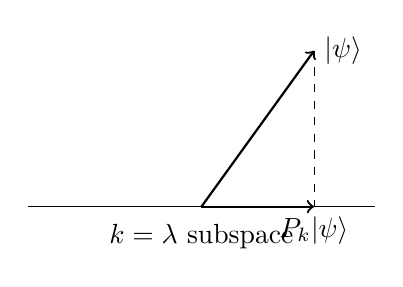
\begin{tikzpicture}[scale=1.1]
\draw (-2,0) -- (2,0);
\draw[->,thick] (0,0) -- (1.3,1.8) node[right] {$|\psi\rangle$};
\draw[dashed] (1.3,1.8) -- (1.3,0);
\draw[->,thick] (0,0) -- (1.3,0) node[below] {$P_k|\psi\rangle$};
\node at (0,-0.35) {$k=\lambda$ subspace};
\end{tikzpicture}\caption{Projektion eines beliebigen Vektors in den Eigenraum \(k=\lambda\).}\end{figure}

\begin{figure}[htbp]\centering
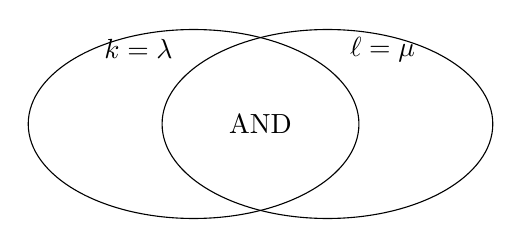
\begin{tikzpicture}[scale=1.0]
\draw (0,0) ellipse (2.1 and 1.2);
\draw (1.7,0) ellipse (2.1 and 1.2);
\node at (-0.7,0.95) {$k=\lambda$};
\node at (2.4,0.95) {$\ell=\mu$};
\node at (0.85,0) {AND};
\end{tikzpicture}\caption{Rekonstruktion der Skizze sich schneidender Unterräume, die der UND-Verknüpfung kommutierender Projektoren zugrunde liegt.}\end{figure}

\begin{figure}[htbp]\centering
\includegraphics[width=0.66\textwidth]{lecture_06_figure_08.png}\caption{Die Tafelherleitung, in der kommutierende Projektoren den gemeinsamen Eigenraum auswählen.}\lectureframe{00:45:20}\end{figure}

\begin{classroomqa}\lecturetimestamp{00:44:42}\audiencequestion{Entspricht die gemeinsame Eigenschaft dem Schnitt im Sinne der klassischen Logik?}\lecturerresponse{Ja. Für kommutierende Projektoren projiziert \(P_kP_\ell\) auf den Schnitt der beiden Eigenräume. Enthält der Schnitt nur den Nullvektor, gibt es keinen von null verschiedenen Zustand mit beiden Eigenschaften.}\end{classroomqa}

Der Vollständigkeit halber lautet der Projektor auf den kompatiblen ODER-Unterraum
\begin{equation}
P_{k\lor\ell}=P_k+P_\ell-P_kP_\ell .
\end{equation}
Sind die Alternativen gegenseitig ausschließend, gilt \(P_kP_\ell=0\), und der Ausdruck vereinfacht sich zur Summe \(P_k+P_\ell\). Diese Subtraktion ist wesentlich, wenn sich die beiden Unterräume überlappen, denn ihr Schnitt darf nicht doppelt gezählt werden.

Anschließend wird die Kompatibilität anhand physikalischer Beispiele erläutert. In einem Zwei-Spin-System kommutiert jede Komponente \(\sigma_i\) des ersten Spins mit jeder Komponente \(\tau_j\) des zweiten:
\begin{equation}
[\sigma_i,\tau_j]=0.
\end{equation}
Dagegen kommutieren verschiedene Komponenten desselben Spins nicht:
\begin{equation}
[\sigma_1,\sigma_3]\neq 0.
\end{equation}
Deshalb kann man je eine Komponente von zwei getrennten Spins messen, aber nicht gleichzeitig zwei verschiedene Komponenten desselben Spins.

\begin{classroomqa}\lecturetimestamp{00:46:12}\audiencequestion{Was sind konkrete Beispiele für kompatible Observablen?}\lecturerresponse{Jeder Operator, der auf den ersten Spin wirkt, kommutiert mit jedem Operator, der auf den zweiten wirkt, da sie auf verschiedene Tensorfaktoren wirken. Auch die Ortskomponenten \(x,y,z\) bilden eine kompatible Familie. Dagegen kommutieren weder zwei verschiedene Komponenten desselben Spins noch Ort und der zugehörige Impuls.}\end{classroomqa}

\begin{classroomqa}\lecturetimestamp{00:47:26}\audiencequestion{Muss ein Teilsystem ein anderes Teilchen sein?}\lecturerresponse{Nein. Gemeint ist eine unabhängig festgelegte Menge von Freiheitsgraden. Verschiedene Teilchen liefern die einfachsten Tensorfaktoren; wenn es die Operatorstruktur zulässt, kann man aber auch verschiedene Freiheitsgrade eines einzelnen Teilchens getrennt behandeln.}\end{classroomqa}

\begin{classroomqa}\lecturetimestamp{00:48:37}\audiencequestion{Was ist ein einfaches Beispiel für ein inkompatibles Paar, wenn so viele Operatoren verschiedener Teilsysteme kommutieren?}\lecturerresponse{Zwei Komponenten desselben Spins sind das Standardbeispiel: \(\sigma_1\) und \(\sigma_3\) kommutieren nicht, sodass kein Messgerät beiden gleichzeitig scharfe Werte zuordnen kann. Der von null verschiedene Matrixkommutator ist das algebraische Kriterium dafür.}\end{classroomqa}

Nun greift Susskind den Satz von Bell erneut auf. Er wiederholt nicht die Rechnung aus der letzten Vorlesung, sondern baut ihre Logik in der neuen Sprache wieder auf. Die klassische Ungleichung lautet in Wahrscheinlichkeitsform
\begin{equation}
P(A\wedge \neg B)+P(B\wedge \neg C)\ge P(A\wedge \neg C).
\end{equation}
Dies ist ein Satz der klassischen Mengenlogik, nicht der Quantenmechanik. Im Singulettzustand sind die Spins entlang jeder gemeinsamen Achse entgegengesetzt ausgerichtet. Daher lässt sich eine NICHT-Aussage über den ersten Spin in die entsprechende positive Aussage über den zweiten umformulieren. So kann man die Ungleichung als Aussage über gemeinsame Eigenschaften eines Zwei-Spin-Systems schreiben.

Lässt man Identitätsoperatoren auf nicht betrachteten Faktoren weg, lauten die in der Vorlesung auftretenden Projektoren auf einzelne Eigenschaften
\begin{equation}
\frac{1+\sigma_3}{2},\qquad
\frac{1+\frac{\tau_1+\tau_3}{\sqrt2}}{2},\qquad
\frac{1+\frac{\sigma_1+\sigma_3}{\sqrt2}}{2},\qquad
\frac{1+\tau_1}{2}.
\end{equation}
Daraus ergeben sich die drei relevanten gemeinsamen Projektoren:
\begin{align}
\Pi_1 &= \frac{1+\sigma_3}{2}\,\frac{1+\frac{\tau_1+\tau_3}{\sqrt2}}{2}, \\
\Pi_2 &= \frac{1+\frac{\sigma_1+\sigma_3}{\sqrt2}}{2}\,\frac{1+\tau_1}{2}, \\
\Pi_3 &= \frac{1+\sigma_3}{2}\,\frac{1+\tau_1}{2}.
\end{align}

\begin{figure}[htbp]\centering
\includegraphics[width=0.68\textwidth]{lecture_06_figure_09.png}\caption{Die drei Analysatorstellungen als Produkte von Ein-Spin-Projektoren.}\lectureframe{01:01:45}\end{figure}

In der Vorlesung wird der Singulettzustand in der vertrauten, nicht normierten Tafelschreibweise angegeben:
\begin{equation}
|\Psi_{\mathrm{singlet}}\rangle \propto |ud\rangle-|du\rangle.
\end{equation}
Das Proportionalitätszeichen genügt hier. Für die Logik kommt es auf den Zustand selbst und insbesondere auf das relative Vorzeichen an, nicht auf die Gesamtnormierung. Berechnet man im Singulettzustand \(\langle \Pi_1\rangle+\langle \Pi_2\rangle\) und \(\langle \Pi_3\rangle\), ergibt sich die Verletzung aus der vorigen Vorlesung. Die wichtige Schlussfolgerung, die Susskind mündlich hervorhebt, lautet: Die Quantenmechanik ist keine als etwas anderes verkleidete klassische Mengenlogik.

\begin{classroomqa}\lecturetimestamp{00:52:31}\audiencequestion{Sind Spin-up und Spin-down orthogonal, bedeutet das Minuszeichen dann, dass das eine Ket das Negative des anderen ist?}\lecturerresponse{Nein. \(|u\rangle\) und \(|d\rangle\) sind verschiedene orthogonale Vektoren. Ein relatives Vorzeichen gehört zu einer Superposition wie \(|ud\rangle-|du\rangle\) und kann deren physikalische Eigenschaften verändern; nur ein Vorzeichen, das den gesamten Zustand multipliziert, ist unerheblich.}\end{classroomqa}

\begin{classroomqa}\lecturetimestamp{00:53:06}\audiencequestion{Wird die Bell-Ungleichung für jeden Quantenzustand und jede Wahl von Eigenschaften verletzt?}\lecturerresponse{Nein. Für viele Zustände und viele Achsenwahlen ist eine bestimmte Bell-Ungleichung erfüllt. Ob sie verletzt wird, hängt sowohl vom Zustand als auch von den ausgewählten Observablen ab. Eine Änderung der Zwischen- und Endwinkel beeinflusst, ob dieser Test die nichtklassischen Korrelationen sichtbar macht.}\end{classroomqa}

\begin{classroomqa}\lecturetimestamp{01:02:47}\audiencequestion{Was lässt sich daraus schließen, dass ein bestimmter Zustand diese Bell-Ungleichung verletzt oder zufällig erfüllt?}\lecturerresponse{Eine Verletzung beweist, dass die beobachteten Statistiken nicht aus der klassischen Mengenlogik hervorgehen können, die der Herleitung zugrunde liegt. Dass eine ausgewählte Ungleichung erfüllt ist, macht den Zustand für sich genommen nicht klassisch, denn bei einer anderen Wahl von Eigenschaften kann eine Verletzung auftreten.}\end{classroomqa}

\section{Lokalität nach Bell}

Die Projektorrechnung ist kein bloßes Spiel mit Symbolen. Man kann sich vorstellen, wiederholt korrelierte Paare im Singulett-Grundzustand vorzubereiten, die beiden Teilchen zu trennen und das identisch präparierte Ensemble in drei große Gruppen aufzuteilen. In der ersten Gruppe misst man die Einstellungen \(0^\circ\) und \(45^\circ\), in der zweiten \(45^\circ\) und \(90^\circ\) und in der dritten \(0^\circ\) und \(90^\circ\). Die Häufigkeiten in den drei Gruppen liefern Schätzungen für die drei Wahrscheinlichkeiten der Ungleichung.

\begin{classroomqa}\lecturetimestamp{01:04:30}\audiencequestion{Welche Versuchsanordnung beschreiben die drei Wahrscheinlichkeiten der Bell-Ungleichung konkret?}\lecturerresponse{Eine Quelle erzeugt viele identisch präparierte verschränkte Paare und schickt deren Teilchen zu räumlich getrennten Analysatoren. Man teilt die Paare in drei Ensembles auf und verwendet für jedes Ensemble das zugehörige Paar von Analysatorrichtungen. Durch Zählen der gemeinsamen Messergebnisse lässt sich jede Wahrscheinlichkeit schätzen. Ein geladenes Teilchen und sein Antiteilchen könnten durch ein Feld getrennt werden; in praktischen Bell-Experimenten verwendet man häufig stattdessen Photonen.}\end{classroomqa}

\begin{classroomqa}\lecturetimestamp{01:08:00}\audiencequestion{Der klassische Mengenbeweis verwendete eine einzige Population. Wie können drei getrennt gemessene Ensembles ihn prüfen?}\lecturerresponse{Die Ungleichung gilt für Wahrscheinlichkeiten ebenso wie für Häufigkeiten. Werden alle drei Stichproben nach demselben Präparationsverfahren gezogen, schätzen ihre relativen Häufigkeiten die drei Wahrscheinlichkeitsverteilungen eines gemeinsamen Ensembles. Die identische Präparation ist die unverzichtbare Voraussetzung.}\end{classroomqa}

Dieser Rückblick auf Bell führt unmittelbar zu der physikalischen Irritation, die noch im Raum steht. Wenn die Korrelationen real sind, warum lassen sie sich dann nicht zur Signalübertragung nutzen?

\begin{classroomqa}\lecturetimestamp{01:09:41}\audiencequestion{Warum lassen sich die Korrelationen verschränkter Teilchen nicht nutzen, um eine überlichtschnelle Nachricht zu senden?}\lecturerresponse{Jede Seite für sich beobachtet weiterhin eine unkontrollierbare Zufallsfolge. Sichtbar wird die Korrelation erst, wenn man die beiden Aufzeichnungen über einen gewöhnlichen klassischen Kanal vergleicht. Bei einem entscheidenden Bell-Test wählt man die Messanordnungen und erfasst die Ergebnisse jedoch so, dass zwischen den beiden Seiten rechtzeitig kein Lichtsignal übermittelt werden könnte. Damit wird ein lokaler Kommunikationsmechanismus als Ursache der gemeinsamen Statistik ausgeschlossen.}\end{classroomqa}

Vergeht genug Zeit, damit ein Lichtsignal zwischen den Apparaturen reisen kann, widerspricht eine Korrelation für sich genommen nicht der Relativitätstheorie; möglicherweise hat man lediglich einen unbemerkten gewöhnlichen Einfluss entdeckt. Das aussagekräftige Experiment schließt diese Ausweichmöglichkeit aus. In Bells Sprache muss eine Theorie mit verborgenen Variablen, die diese Korrelationen reproduziert, nichtlokal sein. Eine nichtlokale Abhängigkeit ist jedoch nicht dasselbe wie eine kontrollierbare überlichtschnelle Nachricht.

\begin{classroomqa}\lecturetimestamp{01:12:18}\audiencequestion{Ist die Drehimpulserhaltung für dieses Argument wesentlich?}\lecturerresponse{Nein. Der Spin ist ein zweckmäßiges Modell mit zwei Zuständen, aber kein unverzichtbarer Bestandteil. Jedes Paar von zweistufigen Systemen mit dem erforderlichen verschränkten Zustand und verschiedenen Messbasen kann dieselbe logische Struktur zeigen.}\end{classroomqa}

Diese Diskussion beendet die Vorlesung nicht, sondern bereitet den nächsten Themenwechsel vor. Bell hat gezeigt, dass die Quantenmechanik keine klassische Logik ist; die nächste Frage ist jedoch eine andere: Was ist eine Messung, operational und mathematisch betrachtet, und wie geht sie in die Interferenz ein?

\section{Doppelspalt mit endlich vielen Zuständen, Interferenz und Messung als Verschränkung}

Nun wechselt die Vorlesung das Modell. Susskind wendet sich dem Doppelspaltversuch zu, vereinfacht ihn aber sofort zu einem Problem mit endlich vielen Zuständen, damit sich dieselben Methoden des Vektorraums nutzen lassen, ohne den vollen mathematischen Apparat der kontinuierlichen Wellenmechanik einzuführen. Sinngemäß sagt er sogar, es handle sich noch immer um den Doppelspaltversuch, nur reduziert auf eine kleine Menge von Basiszuständen.

Es gibt einen Quellzustand \(|0\rangle\), zwei Spaltzustände \(|1\rangle\) und \(|-1\rangle\) sowie eine Menge von Schirmzuständen \(|n\rangle\). Diese \(|n\rangle\) sind orthonormal, weil verschiedene Schirmpositionen verschiedenen Konfigurationen entsprechen. Die Vorlesung lässt die Normierung hier ausdrücklich außer Acht. Die Unitarität wird vorerst zurückgestellt. In diesem Stadium kommt es auf die Linearität an.

\begin{figure}[htbp]\centering
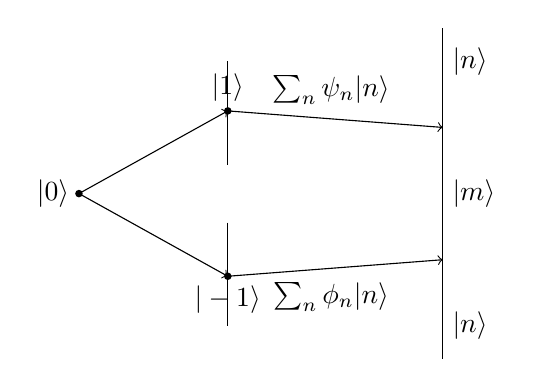
\begin{tikzpicture}[scale=1.05]
\fill (0,0) circle (1.3pt);
\node[left] at (0,0) {$|0\rangle$};

\draw (1.8,1.6) -- (1.8,0.35);
\draw (1.8,-0.35) -- (1.8,-1.6);
\fill (1.8,1) circle (1.3pt);
\fill (1.8,-1) circle (1.3pt);
\node[above] at (1.8,1) {$|1\rangle$};
\node[below] at (1.8,-1) {$|-1\rangle$};

\draw (4.4,2.0) -- (4.4,-2.0);
\node[right] at (4.4,1.6) {$|n\rangle$};
\node[right] at (4.4,0.0) {$|m\rangle$};
\node[right] at (4.4,-1.6) {$|n\rangle$};

\draw[->] (0,0) -- (1.8,1);
\draw[->] (0,0) -- (1.8,-1);
\draw[->] (1.8,1) -- (4.4,0.8);
\draw[->] (1.8,-1) -- (4.4,-0.8);

\node at (3.05,1.25) {$\sum_n \psi_n |n\rangle$};
\node at (3.05,-1.25) {$\sum_n \phi_n |n\rangle$};
\end{tikzpicture}\caption{Eine Version des Doppelspaltversuchs mit endlich vielen Zuständen: der Quellzustand \(|0\rangle\), die beiden Spaltzustände \(|1\rangle\) und \(|-1\rangle\) sowie die Schirmbasis \(|n\rangle\).}\end{figure}

\begin{figure}[htbp]\centering
\includegraphics[width=0.68\textwidth]{lecture_06_figure_10.png}\caption{Das endliche Ortsgitter neben der linearen Entwicklungsvorschrift \(A\to A'\), \(B\to B'\).}\lectureframe{01:18:00}\end{figure}

Aufgrund der Symmetrie entwickelt sich der Quellzustand zu einer gleichgewichteten Superposition der beiden Spaltzustände:
\begin{equation}
|0\rangle \longrightarrow |1\rangle+|-1\rangle.
\end{equation}
Nun entwickle sich der Zustand am oberen Spalt zu
\begin{equation}
|1\rangle \longrightarrow \sum_n \psi_n |n\rangle,
\end{equation}
und derjenige am unteren Spalt zu
\begin{equation}
|-1\rangle \longrightarrow \sum_n \phi_n |n\rangle.
\end{equation}
Die Pfeile bezeichnen hier die Zeitentwicklung, nicht die Gleichheit von Zuständen zum selben Zeitpunkt. Wegen der Linearität gilt
\begin{equation}
|1\rangle+|-1\rangle \longrightarrow \sum_n (\psi_n+\phi_n)|n\rangle.
\end{equation}
Das ist die entscheidende Regel: Die Amplituden addieren sich, bevor man die Wahrscheinlichkeiten bildet.

\begin{classroomqa}
\lecturetimestamp{01:21:59}
\audiencequestion{Wie kann sich der Zustand am Spalt \(|1\rangle\) in Zustände verwandeln, die ebenfalls durch ganze Zahlen \(n\) bezeichnet werden? Sind das Kets am selben Ort und zur selben Zeit?}
\lecturerresponse{Die Bezeichnungen beziehen sich auf verschiedene Zeitpunkte. \(|1\rangle\) bezeichnet das Elektron am oberen Spalt, während die \(|n\rangle\) rechts mögliche spätere Positionen auf dem Schirm bezeichnen. Der Pfeil steht für die zeitliche Entwicklung, nicht für eine Gleichheit zwischen gleichzeitigen Konfigurationen.}
\end{classroomqa}

\begin{classroomqa}
\lecturetimestamp{01:25:30}
\audiencequestion{Müssen die Amplituden normiert sein, und haben sie physikalische Einheiten?}
\lecturerresponse{Eine vollständige zeitliche Entwicklung muss die Gesamtwahrscheinlichkeit erhalten; das ist die Unitarität. Hier wird der gemeinsame Normierungsfaktor weggelassen, weil es nur auf Addition und Auslöschung der Pfadamplituden ankommt. Beliebige Skalierungsfaktoren lassen sich bei der Normierung des Zustands wieder einsetzen.}
\end{classroomqa}

Die Wahrscheinlichkeit, am Schirm den Ort \(m\) zu erreichen, ist daher
\begin{align}
P_m &= |\psi_m+\phi_m|^2 \\
    &= |\psi_m|^2 + |\phi_m|^2 + \psi_m^*\phi_m + \phi_m^*\psi_m.
\end{align}
Die ersten beiden Terme wären auch bei klassischer Betrachtung aufgetreten. Die letzten beiden sind die Interferenzterme.

\begin{figure}[htbp]
\centering
\includegraphics[width=0.68\textwidth]{lecture_06_figure_11.png}
\caption{Die Schirmamplitude und ihre Entwicklung der Wahrscheinlichkeit in vier Terme an der Tafel.}
\lectureframe{01:29:20}
\end{figure}

Am symmetrischen Punkt auf dem Schirm, nennen wir ihn \(m=0\), legt die Symmetrie \(\psi_0=\phi_0\) nahe. Dann gilt
\begin{equation}
P_0 = |\psi_0+\phi_0|^2 = |2\psi_0|^2 = 4|\psi_0|^2.
\end{equation}
Bei geöffneten beiden Spalten ist die Wahrscheinlichkeit an diesem Punkt viermal so groß wie bei nur einem geöffneten Spalt, nicht doppelt so groß. Das ist konstruktive Interferenz.

Nun bringen wir einen Phasenschieber ein, sodass \(\phi_0=-\psi_0\) gilt. Dann
\begin{equation}
P_0 = |\psi_0-\psi_0|^2 = 0.
\end{equation}
Jeder Spalt für sich ermöglicht es dem Elektron, diesen Punkt zu erreichen; werden jedoch beide zugleich geöffnet, kann das Erreichen des Punktes unmöglich werden. Das ist destruktive Interferenz. Susskind verweilt ausdrücklich dabei, wie seltsam das ist: Seiner Ansicht nach ist es so seltsam wie Bells Theorem.

\begin{classroomqa}
\lecturetimestamp{01:33:14}
\audiencequestion{Was geschieht, wenn der Phasenschieber oder die Spaltwahl erst geändert wird, nachdem das Elektron bereits unterwegs ist? Muss der andere Spalt erst davon erfahren?}
\lecturerresponse{Die Antwort hängt von der genauen Raumzeitkonfiguration ab und davon, ob das Elektron dem veränderten Teil des Aufbaus begegnet. Die Quantenmechanik beschreibt die zeitliche Entwicklung des Zustands durch den tatsächlich vorhandenen Aufbau; die Wahrscheinlichkeiten ergeben sich weiterhin aus der Addition der jeweils relevanten Amplituden. Ein verzögertes Wahl-Experiment muss präzise spezifiziert werden, bevor Aussagen über Lokalität beurteilt werden können.}
\end{classroomqa}

Nun führen wir den Aufbau ein. Hinzu kommt ein Zweizustandssystem: ein Spin, der sich anfangs im Zustand \(|d\rangle\) befindet. Geht das Elektron durch den oberen Spalt, kippt es diesen Spin in den Zustand \(|u\rangle\). Geht es durch den unteren Spalt, lässt es ihn unverändert. Der anfängliche zusammengesetzte Zustand ist \(|0,d\rangle\), und die erste Entwicklungsvorschrift lautet nun
\begin{equation}
|0,d\rangle \longrightarrow |1,u\rangle + |-1,d\rangle.
\end{equation}
Diese eine Zeile bringt die Bedeutung der Messung in dieser Vorlesung vollständig auf den Punkt. Die Position des Elektrons ist mit der im Messgerät gespeicherten Aufzeichnung verschränkt worden.

\begin{figure}[htbp]
\centering
\includegraphics[width=0.66\textwidth]{lecture_06_figure_12.png}
\caption{Der Detektorspin korreliert seine Aufzeichnungen „Spin oben“ und „Spin unten“ mit den beiden Spaltalternativen.}
\lectureframe{01:44:10}
\end{figure}

\begin{classroomqa}
\lecturetimestamp{01:40:20}
\audiencequestion{Muss an beiden Spalten ein Detektor stehen?}
\lecturerresponse{Ein zuverlässiger Detektor genügt. Wenn er den Durchgang durch den oberen Spalt aufzeichnet, kennzeichnet eine unveränderte Aufzeichnung die untere Alternative – vorausgesetzt, jedes hindurchtretende Elektron muss eine der beiden Öffnungen passieren. Ein zweiter Detektor ist möglich, fügt aber ein weiteres Teilsystem hinzu, ohne das Prinzip zu ändern.}
\end{classroomqa}

\begin{classroomqa}
\lecturetimestamp{01:40:51}
\audiencequestion{Warum sagt man nicht einfach, dass das Elektron durch beide Spalte geht?}
\lecturerresponse{Ohne eine Aufzeichnung des Weges liegt der Zustand als kohärente Superposition vor; eine nachträgliche Tatsache darüber, welchen Weg das Elektron genommen hat, gibt es nicht. Bei einer vollständigen Welcher-Weg-Messung zeichnet der Aufbau bei jedem Durchgang die eine oder die andere Alternative auf. Was bei beiden Alternativen erhalten bleibt, ist die Zustandsamplitude, nicht etwa zwei getrennt beobachtete Elektronenbahnen.}
\end{classroomqa}

\begin{figure}[htbp]
\centering
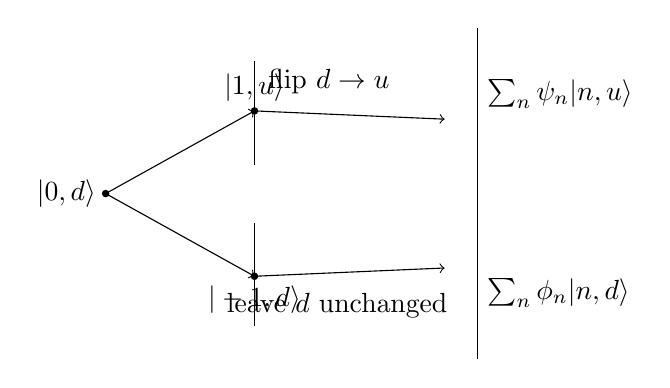
\begin{tikzpicture}[scale=1.05]
\fill (0,0) circle (1.3pt);
\node[left] at (0,0) {$|0,d\rangle$};

\draw (1.8,1.6) -- (1.8,0.35);
\draw (1.8,-0.35) -- (1.8,-1.6);
\fill (1.8,1) circle (1.3pt);
\fill (1.8,-1) circle (1.3pt);
\node[above] at (1.8,1) {$|1,u\rangle$};
\node[below] at (1.8,-1) {$|-1,d\rangle$};

\draw (4.5,2.0) -- (4.5,-2.0);
\node[right] at (4.5,1.2) {$\sum_n \psi_n |n,u\rangle$};
\node[right] at (4.5,-1.2) {$\sum_n \phi_n |n,d\rangle$};

\draw[->] (0,0) -- (1.8,1);
\draw[->] (0,0) -- (1.8,-1);
\draw[->] (1.8,1) -- (4.1,0.9);
\draw[->] (1.8,-1) -- (4.1,-0.9);

\node at (2.7,1.35) {flip \(d\to u\)};
\node at (2.8,-1.35) {leave \(d\) unchanged};
\end{tikzpicture}
\caption{Messung als Verschränkung mit einem Detektorspin. Beim oberen Weg kippt der Spin des Messgeräts, beim unteren bleibt er unverändert.}
\end{figure}

Nehmen wir wie in der Vorlesung an, dass während des Weges zum Schirm nichts Weiteres mit dem Spin geschieht. Dann gilt
\begin{align}
|1,u\rangle &\longrightarrow \sum_n \psi_n |n,u\rangle, \\
|-1,d\rangle &\longrightarrow \sum_n \phi_n |n,d\rangle.
\end{align}
Der Endzustand bei geöffneten beiden Spalten ist daher
\begin{equation}
|\Psi_{\mathrm{final}}\rangle
  = \sum_n \psi_n |n,u\rangle + \sum_n \phi_n |n,d\rangle.
\end{equation}
Dies ist keine Superposition von Zuständen eines einzelnen Elektrons. Es ist ein verschränkter Zustand von Elektron und Messgerät.

\begin{figure}[htbp]
\centering
\includegraphics[width=0.68\textwidth]{lecture_06_figure_13.png}
\caption{Die beiden Pfadamplituden erreichen den Schirm und tragen dabei orthogonale Aufzeichnungen des Messgeräts.}
\lectureframe{01:47:35}
\end{figure}

Am einfachsten berechnet man die Wahrscheinlichkeit, den Ort \(m\) zu erreichen, mithilfe des Projektors auf diesen Ort im Elektron-Teilsystem:
\begin{equation}
\Pi_m = |m\rangle\langle m|\otimes I_{\mathrm{spin}}.
\end{equation}
Die Anwendung von \(\Pi_m\) auf den Endzustand ergibt
\begin{equation}
\Pi_m |\Psi_{\mathrm{final}}\rangle
= |m\rangle\bigl(\psi_m|u\rangle+\phi_m|d\rangle\bigr).
\end{equation}
Die Wahrscheinlichkeit, \(m\) zu erreichen, ist also
\begin{align}
P_m
  &= \langle \Psi_{\mathrm{final}}|\Pi_m|\Psi_{\mathrm{final}}\rangle \\
  &= \bigl(\psi_m^*\langle u|+\phi_m^*\langle d|\bigr)
     \bigl(\psi_m|u\rangle+\phi_m|d\rangle\bigr) \\
  &= |\psi_m|^2 + |\phi_m|^2
     + \psi_m^*\phi_m\langle u|d\rangle
     + \phi_m^*\psi_m\langle d|u\rangle.
\end{align}
Die Aufzeichnungszustände sind jedoch orthogonal:
\begin{equation}
\langle u|d\rangle=0.
\end{equation}
Damit verschwinden die Kreuzterme:
\begin{equation}
P_m = |\psi_m|^2 + |\phi_m|^2.
\end{equation}
Das ist der mathematische Höhepunkt der Vorlesung. Sobald die Welcher-Weg-Information aufgezeichnet ist, verschwindet die Interferenz, und die Wahrscheinlichkeiten addieren sich wie in der klassischen Physik.

\begin{classroomqa}
\lecturetimestamp{01:49:09}
\audiencequestion{Worin besteht der Unterschied zwischen der Superposition \(|1\rangle+|-1\rangle\) und dem Zustand \(|1,u\rangle+|-1,d\rangle\)?}
\lecturerresponse{Im ersten Fall handelt es sich um ein System in einer Linearkombination zweier Positionen; es gibt kein weiteres System, mit dem es verschränkt sein könnte. Im zweiten Fall geht es um zwei Systeme, und der Weg ist mit dem Detektorspin korreliert. Eine Messung des Spins liefert dann Information über den Weg.}
\end{classroomqa}

\section{Aufzeichnungen der Umgebung und partielle Messung}

Nicht nur ein eigens gebauter Detektor kann als Aufzeichnungsgerät dienen. Auch ein Atom nahe einem Spalt, Restgas, eine Wärmequelle oder irgendein anderer Freiheitsgrad kann mit dem Weg korreliert werden. Wenn die Endzustände \(|E_1\rangle\) und \(|E_2\rangle\) sind, hat der Wegzustand die Form
\begin{equation}
|\Psi\rangle
=\sum_n\left(\psi_n|n\rangle|E_1\rangle
+\phi_n|n\rangle|E_2\rangle\right).
\end{equation}
Die Interferenzterme werden nun mit dem Überlapp \(\langle E_1|E_2\rangle\) multipliziert. Bei orthogonalen Aufzeichnungen lassen sich die Wege perfekt unterscheiden, und die Interferenz verschwindet vollständig. Sind die Aufzeichnungen identisch, gilt \(\langle E_1|E_2\rangle=1\), und die Interferenz bleibt erhalten. Bei einem Zwischenwert des Überlapps ist die Sichtbarkeit teilweise erhalten.

\begin{figure}[htbp]
\centering
\includegraphics[width=0.68\textwidth]{lecture_06_figure_14.png}
\caption{Überlappende und getrennte Wellenpakete der Umgebung veranschaulichen partielle und vollständige Aufzeichnungen des Weges.}
\lectureframe{01:53:40}
\end{figure}

\begin{classroomqa}
\lecturetimestamp{01:50:48}
\audiencequestion{Würde ein gewöhnliches Atom in der Nähe des Spalts auch dann mit dem vorbeifliegenden Elektron verschränkt, wenn niemand es absichtlich beobachtet?}
\lecturerresponse{Ja. Entscheidend ist nicht, ob jemand etwas weiß, sondern ob eine physikalische Korrelation entsteht. Wird das Atom oder das umgebende Gas so stark gestört, dass sein späterer Zustand den Weg erkennen lässt, zeichnet es Welcher-Weg-Information auf und unterdrückt die Interferenz. Deshalb müssen solche Experimente isoliert und bei niedrigen Temperaturen durchgeführt werden; oft verwendet man außerdem schwach wechselwirkende Teilchen wie Photonen.}
\end{classroomqa}

Durch Abkühlung befinden sich die Freiheitsgrade der Umgebung nahe ihren Grundzuständen, wodurch unbeabsichtigte Aufzeichnungen seltener werden. Auch eine Energielücke hilft: Kann das einfallende Teilchen nicht die Mindestanregungsenergie liefern, ist die Umgebung möglicherweise nicht in der Lage, Weg-Information festzuhalten. Geladene Teilchen hingegen können die Materie in ihrer Nähe durch ihre elektrischen Felder stören, was Interferenzexperimente mit Elektronen besonders anspruchsvoll macht.

\begin{classroomqa}
\lecturetimestamp{01:54:49}
\audiencequestion{Kann man tatsächlich mit einzelnen Elektronen ein Interferenzmuster erzeugen?}Jedes Elektron erzeugt nur einen einzelnen, lokalisierten Treffer. Lässt man die Teilchen einzeln und mit genügend großem Abstand passieren, sodass sie nicht miteinander wechselwirken können, und wiederholt das Experiment oft, zeigt die resultierende Häufigkeitsverteilung das Interferenzmuster. Ein einzelnes Ereignis ist nur ein kleiner Fleck.\lecturerresponse{
}
\end{classroomqa}

\begin{classroomqa}
\lecturetimestamp{01:55:59}
\audiencequestion{Zerstört eine Messung Verschränkung, oder erzeugt sie sie?}
\lecturerresponse{Die Welcher-Weg-Wechselwirkung erzeugt eine Verschränkung zwischen System und Messgerät und zerstört dadurch die Interferenz zwischen den Alternativen. Eine spätere Messung kann das Messgerät mit einem weiteren System korrelieren und den verbleibenden Zustand gegebenenfalls bedingt festlegen. Deshalb muss man immer angeben, um welche beiden Teilsysteme und um welche Interferenz es geht.}
\end{classroomqa}

\begin{classroomqa}
\lecturetimestamp{01:57:44}
\audiencequestion{Lässt sich die Wechselwirkung so abschwächen, dass das Messgerät nur teilweise Information über den Weg erhält?}
\lecturerresponse{Ja. Bei einer schwachen Wechselwirkung kippt der Detektor möglicherweise nur mit einer bestimmten Amplitude, sodass die Aufzeichnungszustände nicht orthogonal bleiben. Dann lassen sich die Wege nur teilweise unterscheiden, und die Interferenz wird nur teilweise abgeschwächt. Je stärker die Messung ist, desto besser lassen sich die Wege unterscheiden, desto stärker ist die Verschränkung mit der Aufzeichnung und desto geringer die Sichtbarkeit der Streifen.}
\end{classroomqa}

Der hier gemeinte Kollaps ist also konkret: Er besteht im Verlust der Kreuzterme, wenn die Weg-Information in einem anderen System gespeichert wurde. Ohne Aufzeichnung addieren sich die Amplituden. Bei perfekt unterscheidbaren Aufzeichnungen verschwinden ihre Skalarprodukte, und die Wahrscheinlichkeiten addieren sich. Zwischen diesen beiden Grenzfällen ändern sich Messstärke und Interferenzsichtbarkeit kontinuierlich.
